\chapter{Reconoces las propiedades de los polígonos}

\section{Polígonos}

\subsection{Definición}

Wikipedia da las definiciones siguientes:

\begin{itemize}
\item Un polígono es una figura plana compuesta por una secuencia finita de
segmentos rectos consecutivos que cierran una región en el plano.
\item Un polígono es simple, si ningún par de aristas no consecutivas se corta.
  Equivalentemente, su frontera tiene un solo contorno.
\item Complejo, si dos de sus aristas no consecutivas se intersecan
\item Convexo, si tiene todos sus ángulos internos menores que 180º. O bien,
  si un segmento que une dos puntos cualesquiera del polígono yace en el
  interior de este.
\item Cóncavo, si al atravesarlo una recta puede cortarlo en más de dos puntos; es el que tiene uno o varios ángulos mayores que 180º.
\item Regular, si tiene todos sus lados iguales y todos sus ángulos iguales.
\item Un polígono con $n$ lado se llama un $n$-gono y para diferentes valor de
  $n$, dicemos que es un triángulo (3 lados), cuadrilátero (4 lados), pentágono
(5 lados), hexágono (6 lados), heptágono (7 lados), octógono (8 lados),
decágono (10 lados), dodecágono (12 lados) etc
\end{itemize}

\subsection{Ejercicio 1}

Indique si los figuras siguientes son polígonos.

\begin{enumerate}

\item
 \begin{tikzpicture}
   \draw (0,0) -- (1,0) -- (2,1) -- (1,2);
 \end{tikzpicture}

\item
  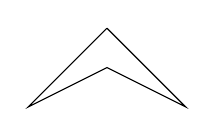
\begin{tikzpicture}
    \draw(1,1) --(0,0) -- (1,.5) -- (2,0) -- (1,1);
  \end{tikzpicture}

\item 
 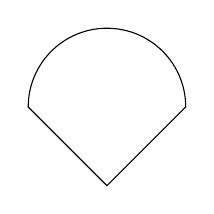
\begin{tikzpicture}
   \draw (0,0) -- (1,-1) -- (2,0) arc (0:180:1);
 \end{tikzpicture}

\item 
 \begin{tikzpicture}
   \draw (0,0) node[left]{$(0,0)$} --
   (0,2)node[above left]{$(0,2)$} --
   (6,2)node[above left]{$(6,2)$} --
   (8,4)node[above right]{$(8,4)$} --
   (4,-2)node[below]{$(4,-2)$} --
   (2,1)node[above]{$(2,1)$} --
   (1,-.5)node[below]{$\left(\frac{8}{2^n}, {(-1)}^n \frac{4}{2^n} \right)$} --
   (.5,.25);
   \draw (.5,.25) -- (.25,-.125)[dashed];
 \end{tikzpicture}

\item 
  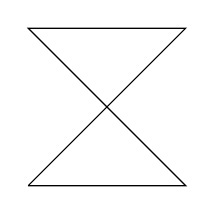
\begin{tikzpicture}
    \draw(0,0) --(2,0) -- (0,2) -- (2,2) -- (0,0);
  \end{tikzpicture}


\end{enumerate}

\subsection{Ejercicio 2}

Sean $A,B,C,D,E,G,G,H,I$ los puntos de coordenadas
$(0,0)$, $(1,0)$, $(2,0)$,
$(0,1)$, $(1,1)$, $(2,1)$,
$(0,2)$, $(1,2)$ y $(2,2)$. Dibuja y describe los polígonos siguientes:

\begin{enumerate}
  \item $AHFBD$
  \item $DBFH$
  \item $ABIHE$
  \item $DBFG$
  \item $BCIH$
\end{enumerate}

\subsection{Cuadriláteros}

Un cuadrilátero que tiene un par de lados paralelos es un trapezoide. Si
los lados opuestos son iguales y paralelos dos a dos, es llamado un
paralelogramo. Un paralelogramo con los cuatros lados paralelos es llamado
un rombo.

Un rectángulo tiene sus 4 ángulos de 90° y entonces es un
paralelogramo. Un cuadrado es un rectángulo con sus cuatro lados iguales y
por lo tanto es un cuadrilátero regular. 

\subsection{Ejercicio 3}

Dibuje:

\begin{enumerate}
\item un cuadrilátero simple convexo que no es un trapezoide.
\item un trapezoide que no es un paralelogramo.
\item un paralelogramo que es ni un rombo, ni un rectángulo.
\item un rombo que no es un cuadrado.
\item un rectángulo que no es un cuadrado.
\item un cuadrado.
\end{enumerate}

\section{Elementos y Propiedades}

\subsection{Definición}

Wikipedia da las definiciones siguientes:

\begin{itemize}
\item Lado: es cada uno de los segmentos que conforman el polígono.
\item Vértice: es el punto de intersección (punto de unión) de dos lados consecutivos.
\item Diagonal: es el segmento que une dos vértices no consecutivos.
\item Ángulo interior de un polígono simple: es el ángulo formado, internamente al polígono, por dos lados consecutivos.
\item Ángulo exterior de un polígono simple convexo: es el ángulo formado,
  externalmente al polígono,
  por un lado y la prolongación de un lado consecutivo.
\item Centro de un polígono regular: es el punto equidistante de todos los vértices y lados.
\item Ángulo central de un polígono regular:
  es el formado por dos segmentos de recta que parten del centro a los extremos
  de un lado.
\item Apotema de un polígono regular: es el segmento que une el centro del polígono con el centro de un lado; es perpendicular a dicho lado.
\end{itemize}

\subsection{Ejercicio 4}

Consideramos un polígono con $n \geq 3$ lados.

\begin{itemize}
\item ¿Cuantos vértices tiene?
\item ¿Cuantos diagonales tiene?
\item ¿Si es regular, cual es la medida de un ángulo central minimal?
  ¿Y la suma de esos ángulos centrales?
\end{itemize}

\subsection{Ejercicio 5}

\begin{itemize}
\item Represente sobre una figura los ángulos interiores y exteriores de
  un triángulo.
\item Recuerde cual es la suma de los ángulos interiores de un triángulo.
\item Deduzca la suma de los ángulos exteriores de un triángulo.
\item Sean $A, B, C$ tres vértices consecutivos de un $n$-gono
  simple convexo ($n \geq 4$).
  Represente sobre una figura los ángulos interiores y exteriores
  $\alpha, \beta, \gamma$
  en $A, B, C$.
\item Si retiramos el punto $B$, exprese la suma de los nuevos
  ángulos exteriores en $A$ y $C$.
\item Deduzca la suma de los ángulos exteriores de un poligóno simple convexo.
\item Exprese la suma de los angúlos interiores del $n-1$-gono ($B$ retirado).
  en función de la suma de los angúlos interiores del $n$-gono.
\item Deduzca la suma de los ángulos interior de un poligóno simple convexo.
\end{itemize}

\subsection{Ejercicio 6 (polígonos regulares)}

Utilice la regla y el compás para construir:

\begin{enumerate}
\item Un círculo $C$ de radio $R=4$.
\item Dos rectas ortogonales que se intersectan en el centro de $C$ (utilice
  la construcción de un mediatriz)
\item Un cuadrado inscrito en $C$.
\item Un polígono regular de lado $R$ y inscrito en $C$. ¿Cómo se llama?
\item Un triángulo equilátero inscrito en $C$.
  Sea $\beta$ un ángulo central de amplitud minimal.
\item La longitud $a=\sqrt{5} - 1$ (ver ejercicio 8 del capítulo III) y
  $b = R - a$.
\item El triángulo rectángulo con un lado menor $a = \sqrt{5} - 1$ y hipotenusa
  $R$. Sea $c$ el otro lado menor.
\item El triángulo rectángulo de catetos $b, c$. Sea $d$ su hipotenusa.
\item Un polígono regular de lado $d$ inscrito en $C$.
  ¿Cómo se llama? Sea $\alpha$ un ángulo central de amplitud minimal.
\item Dos polígonos regulares inscritos en $C$ de ángulos centrales minimales
  $\frac{\alpha}{2}$ y $\frac{\beta}{2}$ (construir las bisectrices de los
  ángulos $\alpha, \beta$). ¿Cómo se llaman?
\item Un octógono y hexadecágono ($16$-gono) regulares inscritos en $C$.
\item Un polígono regular inscrito en $C$ y
  ángulo central minimal $2 \alpha - \beta$. ¿Cómo se llama?
\end{enumerate}

\section{Perímetro y Área}

\subsection{Definición}

La suma de las longitudes los lados del polígono se llama el perímetro.
El tamaño de la región encerrada en el polígono se llama el área.

Por ejemplo, un rectángulo de lados $a,b$ tiene perímetro
$a+b+a+b=2{(a+b)}$ y área $a \times b$.

\begin{center}
 \begin{tikzpicture}
   \draw[color=red] (0,0) -- (2,0)node[below]{$a$} --
   (4,0) -- (4,1)node[right]{$b$} --
   (4,2) -- (2,2)node[above]{$a$} --
   (0,2) -- (0,1)node[left]{$b$} --
   (0,0);
 \end{tikzpicture}
\end{center}

\subsection{Ejercicio 7 (Cuadriláteros)}

\begin{enumerate}
\item
 ¿Cual es el perímetro y área de un cuadrado de lado $a$?

\begin{center}
 \begin{tikzpicture}
   \draw[color=red] (0,0) --
   (2,0) -- (2,1)node[right]{$a$} --
   (2,2) --
   (0,2) --
   (0,0);
 \end{tikzpicture}
\end{center}

\item Sean $a,b$ las longitudes de las diagonales de un rombo y $c$ la de
  un lado. Exprese el perímetro del rombo en función de $c$ y
  el área del rombo en función de $a,b$ (utilice el área del rectángulo ázul)?
  
\begin{center}
 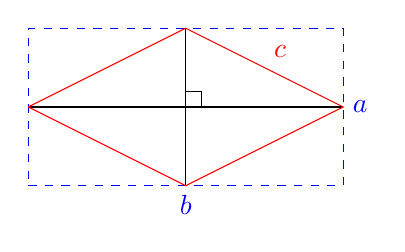
\begin{tikzpicture}
   \draw (2.2,0) -- (2.2,.2) -- (2,.2);
   \draw (0,0) -- (4,0);
   \draw (2,-1) -- (2,1);
   \draw[dashed,color=blue] (0,-1) --
   (2,-1)node[below]{$b$} --
   (4,-1) -- (4,0)node[right]{$a$} -- (4,1) -- (0,1) -- (0,-1);
   \draw[color=red] (0,0) -- (2,-1) -- (4,0) -- (3,.5)node[above right]{$c$} --
   (2,1) -- (0,0);
 \end{tikzpicture}
\end{center}

\item Sean $a,b$ las longitudes de un lado de un paralelogramo y $h$ la
  distancia entre los dos lados paralelos de longitud $a$. 
  Exprese el perímetro del paralelogramo en función de $a,b$ y
  el área del paralelogramo en función de $a,h$.

\begin{center}
 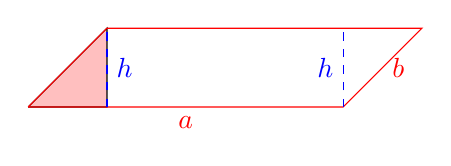
\begin{tikzpicture}
   \draw[color=transparent,fill=pink] (0,0) -- (1,0) -- (1,1) -- (0,0);
   \draw[color=red] (0,0) -- (2,0)node[below]{$a$} --
   (4,0) -- (4.5,.5)node[right]{$b$} -- (5,1) -- (1,1) -- (0,0);
   \draw[dashed,color=blue] (1,0) -- (1,.5)node[right]{$h$} -- (1,1);
   \draw[dashed,color=blue] (4,0) -- (4,.5)node[left]{$h$} -- (4,1);
 \end{tikzpicture}
\end{center}

\item Sean $a,b$ las longitudes de los lados paralelos de un trapezoide y $h$ la
  distancia entre los dos lados.
  Exprese el área del trapezoide en función de $a,b,h$ (utilice el grán
  paralelogramo formado por dos copías del trapezoide).

\begin{center}
 \begin{tikzpicture}
   \begin{scope}[rotate around={180:(3.75,.5)}]
   \draw[dashed,color=red] (0,0) --
   (4,0) -- (3.5,1) -- (1,1) -- (0,0);
   \end{scope}

   \draw[color=red] (0,0) -- (2,0)node[below]{$a$} --
   (4,0) -- (3.5,1) -- (2.5,1)node[above]{$b$} -- (1,1) -- (0,0);

   \draw[dashed,color=blue] (1,0) -- (1,.5)node[right]{$h$} -- (1,1);
 \end{tikzpicture}
\end{center}

\begin{center}
 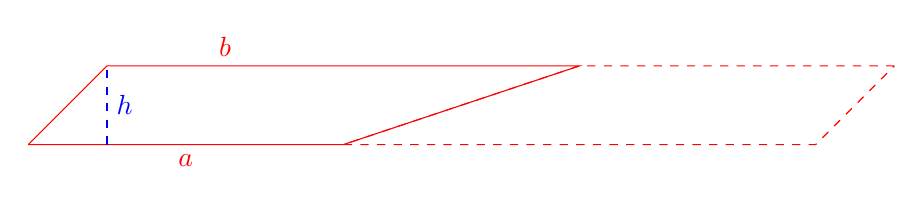
\begin{tikzpicture}
   \begin{scope}[rotate around={180:(5.5,.5)}]
   \draw[dashed,color=red] (0,0) --
   (4,0) -- (7,1) -- (1,1) -- (0,0);
   \end{scope}

   \draw[color=red] (0,0) -- (2,0)node[below]{$a$} --
   (4,0) -- (7,1) -- (2.5,1)node[above]{$b$} -- (1,1) -- (0,0);

   \draw[dashed,color=blue] (1,0) -- (1,.5)node[right]{$h$} -- (1,1);
 \end{tikzpicture}
\end{center}

\end{enumerate}

\subsection{Ejercicio 8 (Triángulo)}

\begin{enumerate}
\item Exprese el perímetro de un triángulo de lados $a,b,c$.
\item Formule expresiones del perímetro para un triángulo isósceles,
  equilátero, rectángulo o isósceles rectángulo.
\item Exprese el área de un triángulo de lado $a$ y altura $h$. 
\begin{center}
 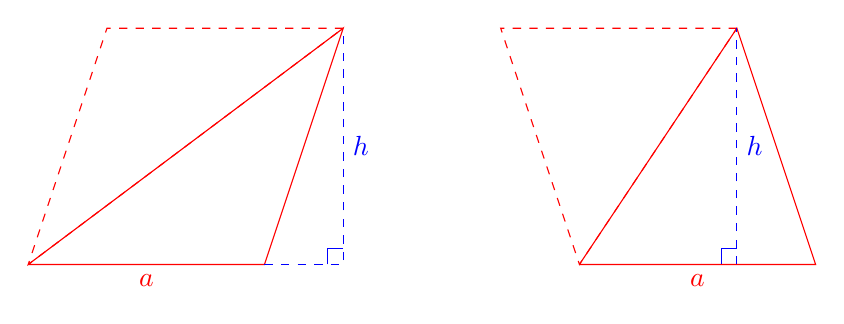
\begin{tikzpicture}
   \draw[color=red]
   (0,0) -- (1.5,0)node[below]{$a$} -- (3,0) -- (4,3) -- (0,0);

   \begin{scope}[rotate around={180:(2,1.5)}]
   \draw[color=red,dashed]
   (0,0) -- (1.5,0) -- (3,0) -- (4,3) -- (0,0);
   \end{scope}
   \draw[color=blue,dashed](3,0)--(4,0)--(4,1.5)node[right]{$h$}--(4,3);
   \draw[color=blue](3.8,0)--(3.8,.2)--(4,.2);

   \begin{scope}[shift={(7,0)}]
     \draw[color=red]
     (0,0) -- (1.5,0)node[below]{$a$} -- (3,0) -- (2,3) -- (0,0);
     \begin{scope}[rotate around={180:(1,1.5)}]
     \draw[color=red,dashed]
     (0,0) -- (3,0) -- (2,3) -- (0,0);
     \end{scope}
     \draw[color=blue,dashed](2,0)--(2,1.5)node[right]{$h$}--(2,3);
   \draw[color=blue](1.8,0)--(1.8,.2)--(2,.2);
   \end{scope}
 \end{tikzpicture}
\end{center}
\item Formule expresiones del área para un triángulo rectángulo,
  isósceles rectángulo o equilátero.
 \end{enumerate}

\subsection{Ejercicio 9 (polígonos regulares, Arquímedes)}

\begin{enumerate}
\item Utilice la regla y el compás para construir: un círculo de centro $O$
  y radio $R$, el hexágono regular $ABCDEF$ de lado $R$ y inscrito en $C$,
  los radios ${OA}, {OB}, \ldots, {OF}$ y los seis apotemas del hexágono.
\item Exprese el périmetro, la longitud del apotema
   y el área del hexágono en función de $R$.
\item Consideramos el hexágono circunscrito a $C$, cuyos los apotemas
  son ${OA}, {OB}, \ldots, {OF}$. ¿Cual es su périmetro y
  área? Deduzca un aproximación del périmetro $P_C$ y área $A_C$ del círculo.
\item Suponemos que el périmetro del círculo es proporcional a la longitud
  de su radio $P_C = 2 \pi R$. Indique una aproximación de la constante $\pi$.
\item De manera general, si consideramos un polígono regular con $n \neq 6$
  lados de lado $l$ y apotema $h$, ¿Cuales son las formulas de périmetro y área?
\item Si tomamos $n$ muy largo, el perímetro del $n$-gono se acerca del
  perímetro del $P_C$, el apotema $h$ se acerca del radio $R$ y
  el área del $n$-gono se acerca del área $A_C$.
  Proponga una formula para el área $A_C$ del círculo en función de $R,\pi$.
\end{enumerate}

\section{Soluciones de los ejercicios}

\subsection{Ejercicio 1}

\begin{enumerate}

\item No (no cierra una región del plano).
\item Si (Polígono cóncavo)
\item No (tiene un segmento que no es recto)
\item No (tiene una infinitad de segmentos)
\item Si (Polígono complejo)
\end{enumerate}

\subsection{Ejercicio 2}

\begin{enumerate}
  \item Pentágono, complejo ($DB$ y $AH$ se intersectan).
  \item Cuadrilátero, simple, convexo, regular (cuadrado).
  \item Pentágono, simple, cóncavo (la amplitud de $\widehat{HEA}$ es
    más que 180°)
  \item Pentágono, simple, convexo ($DB \neq GF$).
\end{enumerate}

\subsection{Ejercicio 3}

\begin{enumerate}
\item 
 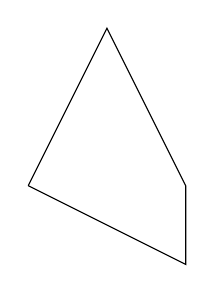
\begin{tikzpicture}
   \draw (0,0) -- (1,2) -- (2,0) -- (2,-1) -- (0,0);
 \end{tikzpicture}

\item 
 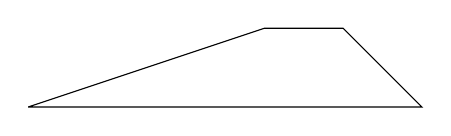
\begin{tikzpicture}
  \draw (0,0) -- (5,0) -- (4,1) -- (3,1) -- (0,0);
 \end{tikzpicture}
\item
 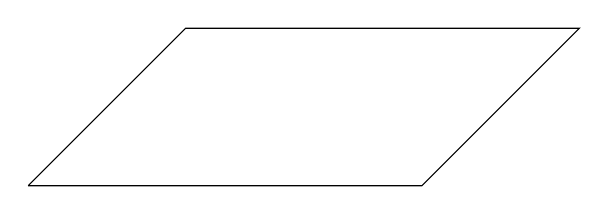
\begin{tikzpicture}
  \draw (0,0) -- (5,0) -- (7,2) -- (2,2) -- (0,0);
 \end{tikzpicture}
\item
 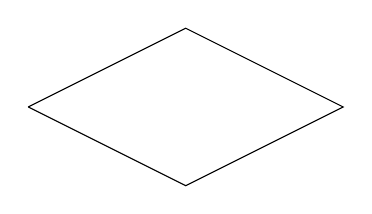
\begin{tikzpicture}
  \draw (0,0) -- (2,-1) -- (4,0) -- (2,1) -- (0,0);
 \end{tikzpicture}
\item 
 \begin{tikzpicture}
  \draw (0,0) -- (4,0) -- (4,2) -- (0,2) -- (0,0);
 \end{tikzpicture}
\item
  Por ejemplo
 \begin{tikzpicture}
  \draw (0,0) -- (2,0) -- (2,2) -- (0,2) -- (0,0);
 \end{tikzpicture}, o con otra orientación:
 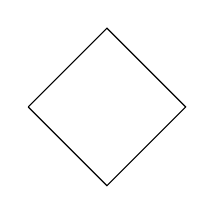
\begin{tikzpicture}
  \draw (0,0) -- (1,-1) -- (2,0) -- (1,1) -- (0,0);
 \end{tikzpicture}
\end{enumerate}

\subsection{Ejercicio 4}

\begin{itemize}
\item Hay dos vértices para cada lados, y cada vértice apartene a dos lados
  entonces hay $\frac{2n}{2} = n$ vértices. Podemos también decir los
  vértices son exactamente los puntos de salida (o de llegada) de los
  lados, y entonces hay $n$ vértices. Por ejemplo, un triángulo tiene tres
  vértices, un cuadrilatero cuatro vértices etc
\item Para obtener un diagonal, elegimos un punto ($n$ posibilidades) y
  otro que no es conectado con el primer ($n-3$ posibilidades). Para cada
  diagonal hay dos posibilidades para el primer punto elegido y entonces
  hay $\frac{n{(n-3)}}{2}$ diagonales. Por ejemplo, un triángulo no tiene 
  diagonal, un cuadrilatero tiene dos diagonales, un pentágono tiene
  cinco diagonales etc
\item Una vuelta completa es 360°. Para un ángulo central (minimal), sólo
  es $\frac{1}{n}$ de una vuelta completa, es decir $\frac{360}{n}$. La suma
  de esos ángulos centrales es 360°.
\end{itemize}

\subsection{Ejercicio 5}

Los ángulos rojos son los ángulos interiores y
los ángulos azules son los ángulos exteriores. La suma de los ángulos interiores
es $x+y+z=180°$.
Además, cada par de ángulo interior/exterior coresponde a
ángulos suplementarios. Entonces la suma de los ángulos exteriores es
${(180° - x)} + {(180° - y)} + {(180° - z)} = 3\times180° - {(x+y+z)} = 360°$.

\begin{center}
 \begin{tikzpicture}
   \draw (0,0) -- (3,0) -- (2,1) -- (0,0);
   \draw[dashed] (3,0) -- (4,-1);
   \draw[dashed] (2,1) -- (4,2);
   \draw[dashed] (0,0) -- (-2,0);

   \draw[color=red](.5,0) arc(0:26:.5) node(A){};
   \draw[color=blue](A) arc(26:180:.5);

   \draw[color=blue](2.5,0) arc(180:316:.5);
   \draw[color=red](2.5,0) arc(180:136:.5);

   \draw[color=blue](2.449397023149583,1.219185573394538) arc(26:-43:.5) node(B){};
   \draw[color=red](B) arc(-43:-152:.5);

 \end{tikzpicture}
\end{center}

Los ángulos rojos son los ángulos interiores y los
ángulos azules son los ángulos exteriores.

\begin{center}
 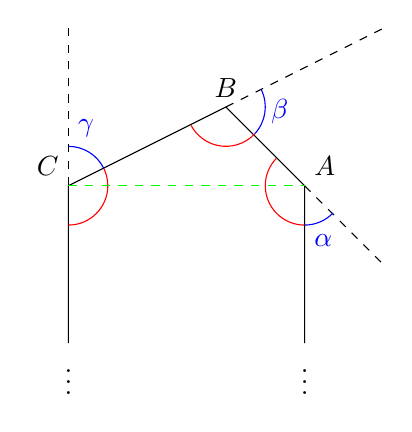
\begin{tikzpicture}
   \draw (0,-2)node[below]{$\vdots$} -- (0,0)node[above left]{$C$} -- (2,1)
   node[above]{$B$} -- (3,0)node[above right]{$A$} --
   (3,-2)node[below]{$\vdots$};
   \draw[dashed] (3,0) -- (4,-1);
   \draw[dashed] (2,1) -- (4,2);
   \draw[dashed] (0,0) -- (0,2);

   \draw[color=red](0,-.5) arc(-90:26:.5) node(A){};
   \draw[color=blue](A) arc(26:90:.5) node[above right]{$\gamma$};

   \draw[color=blue](3,-.5)node[below right]{$\alpha$} arc(270:316:.5);
   \draw[color=red](3,-.5) arc(270:136:.5);

   \draw[color=blue](2.449397023149583,1.219185573394538)
   node[below right]{$\beta$} arc(26:-43:.5) node(B){};
   \draw[color=red](B) arc(-43:-152:.5);

   \draw[dashed,color=green] (0,0) -- (3,0);

 \end{tikzpicture}
\end{center}

Si retiramos el punto $B$, la amplitud del ángulo exterior en $A$ se vuelve
$\alpha + \widehat{CAB}$ y la amplitud del ángulo exterior en $C$ se vuelve
$\gamma + \widehat{BCA}$. Entonces la suma de estes dos ángulos es
$\alpha + \gamma + \widehat{CAB} + \widehat{BCA} =
\alpha + \gamma + {(180° - \widehat{ABC})} = \alpha+\beta+\gamma$.
Por lo tanto, la suma de los ángulos exteriores de un
$n$-gono es la misma que la suma de los angúlos interiores de un $n-1$-gono,
de un $n-2$-gono, $n-3$-gono... y finalmente de un triángulo es decir 360°.

De la misma manera, para obtener la suma de los angúlos interiores en el
$n-1$-gono a partir de la suma del $n$-gono,
restamos el ángulo interior $\widehat{ABC}$,
restamos $\widehat{CAB}$ del ángulo interior en $A$ y
restamos $\widehat{BCA}$ del ángulo interior en $C$. Entonces restamos
$\widehat{ABC}+\widehat{CAB}+\widehat{BCA}=180°$. Al final,
la suma de los ángulos interiores de un triángulo es $180°$, la de un
cuadrado $180+180=360°$, ... y la de un $n$-gono $180\times {(n-2)}$°.

Note que las definiciones y resultados pueden ser generalizados a polígonos
que no son simple o convexo.

\subsection{Ejercicio 6 (polígonos regulares)}

Trazamos el círculo $C$ (azul) con el compás. Con la regla trazamos una recta
pasando por el centro de $C$. Cómo en el ejercicio 5 del capítulo III,
trazamos la recta ortogonal pasando por $C$. Los puntos de interseción de estas
rectas con el círculo $C$ son los cuatros vértice de un cuadrado inscrito en
$C$ (rojo). 

Trazamos con el compás el círculo de centro un punto de $C$ y radio $R$.
Intersecta $C$ en un nuevo punto. Si repetamos esta operación otras veces,
obtenemos un hexágono regular inscrito en $C$ (verde). Tomando un punto sobre
dos de este hexágono, obetemos un triángulo equilátero inscrito en $C$
(naranja).

\begin{center}
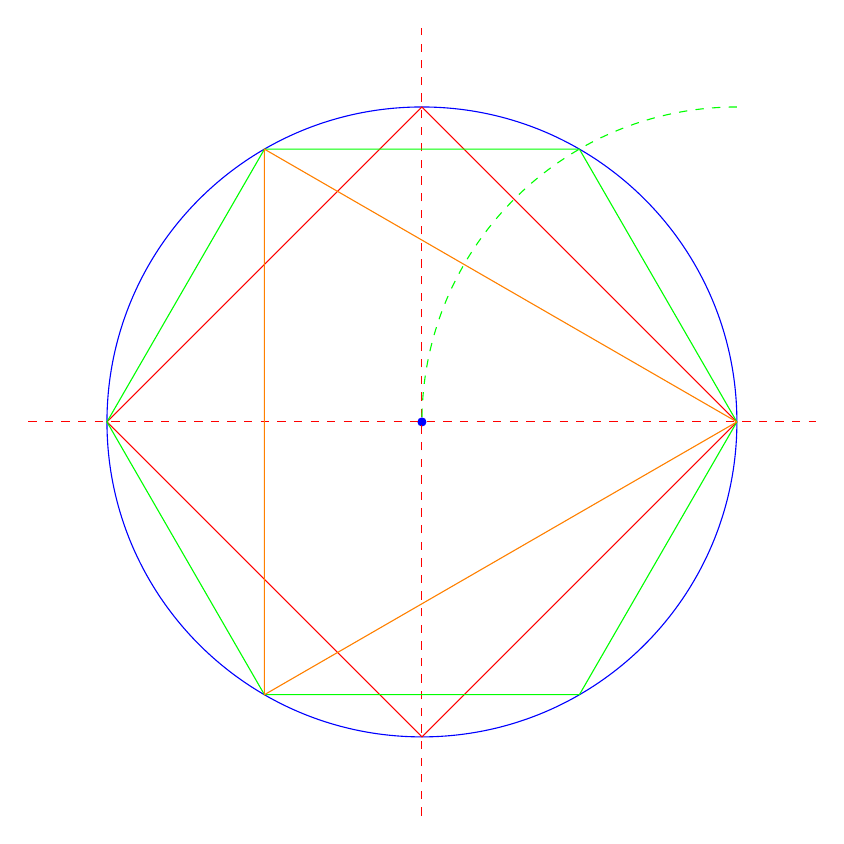
\begin{tikzpicture}
  \draw (0,0) circle(4)[color=blue];
  \draw[fill=black] (0,0) circle(.05)[color=blue];
  \draw (-5,0) -- (5,0)[dashed,color=red];
  \draw (0,-5) -- (0,5)[dashed,color=red];
  \draw (4,0) -- (0,4) -- (-4,0) -- (0,-4) -- (4,0)[color=red];
  \draw (4,4) arc(90:180:4)[dashed,color=green];
  \draw (4,0) -- (2,3.464101615137754) -- (-2,3.464101615137754) --
  (-4,0) -- (-2,-3.464101615137754) -- (2,-3.464101615137754) -- (4,0)
        [color=green];
  \draw (4,0) -- (-2,3.464101615137754) -- (-2,-3.464101615137754) -- (4,0)
        [color=orange];
\end{tikzpicture}
\end{center}

Cómo en el ejercicio 8 del capítulo III, podemos construir la longitud
$\sqrt{5}$ y
entonces $a = \sqrt{5} - 1$ y $b = R - a$. Utilizamos la técnica de la mediatriz
para construir los dos triángulos rectángulos. Repetamos la longitud $d$ con
el compás para obtener un pentágono regular inscrito en $C$ (verde).

\begin{center}
\begin{tikzpicture}
  \draw (0,0) circle(4)[color=blue];
  \draw[fill=black] (0,0) circle(.05)[color=blue];
  \draw (-5,0) -- (5,0)[dashed,color=red];
  \draw (0,-5) -- (0,5)[dashed,color=red];
  \draw[fill=black] (2.23606797749979,0) circle(.05);
  \draw[dashed, color=orange] (2.23606797749979,0) -- (2.23606797749979,-.2) --
  (1.78606797749979,-.2) node[below]{$1$} -- (1.23606797749979,-.2) --
  (1.23606797749979,0);
  \draw[fill=black] (1.23606797749979,0) circle(.05);
  \draw[color=green](0,0) -- (.6,0) node[above]{$a$} --
  (1.23606797749979, 0) -- 
  (1.23606797749979, 1.9)node[right]{$c$} -- 
  (1.23606797749979,3.804226065180614) --
  (.6, 1.9)node[above left]{$R$} -- (0,0);
  \draw[color=green] (1.23606797749979, 0) --
  (2.5,0) node[above]{$b$} -- (4,0) -- 
  (2.618033988749894,1.902113032590307)node[above right]{$d$} --
  (1.23606797749979,3.804226065180614);
  \draw[color=green](1.43606797749979,0) --
  (1.43606797749979,.2) -- (1.23606797749979,.2);
  \draw[color=green]
  (1.23606797749979,3.804226065180614) --
  (-3.236067977499789,2.351141009169893) --
  (-3.23606797749979,-2.351141009169892) --
  (1.23606797749979,-3.804226065180614) -- (4, 0);
  \draw(2.23606797749979,0) -- (3,-1) node[below]{$(\sqrt{5},0)$};

\end{tikzpicture}
\end{center}

Construyendo las mediatrices de los lados del pentágono (es decir las
bisecrices de sus ángulos centrales) obtenemos un decágono regular (naranja)
inscrito en $C$. De la misma manera, a partir del cuadrado y hexágono
obtenemos octógono y dodecágono regulares inscritos en $C$. Y a partir del
octógono, obtenemos un hexadecágono.

\begin{center}
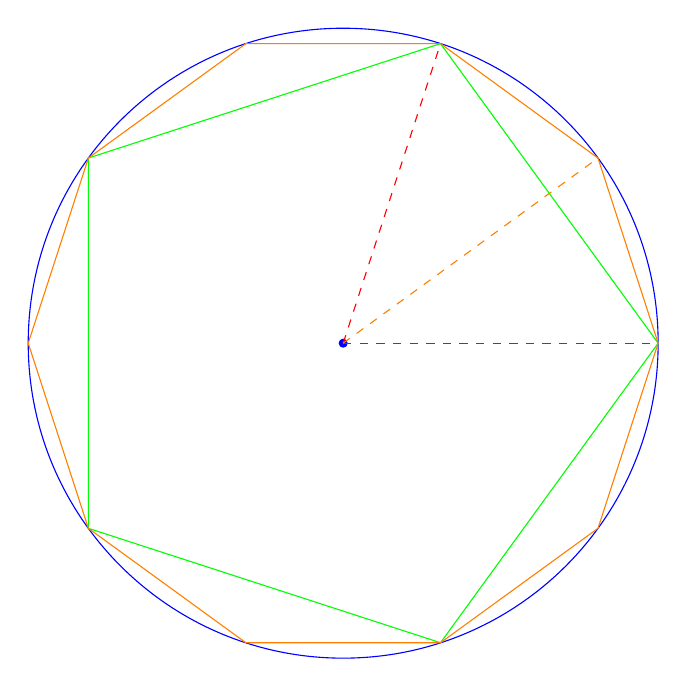
\begin{tikzpicture}
  \draw (0,0) circle(4)[color=blue];
  \draw[fill=black] (0,0) circle(.05)[color=blue];
  \draw[color=green]
  (1.23606797749979,3.804226065180614) --
  (-3.236067977499789,2.351141009169893) --
  (-3.23606797749979,-2.351141009169892) --
  (1.23606797749979,-3.804226065180614) -- (4, 0) --
  (1.23606797749979,3.804226065180614);
  \draw[dashed,color=red] (0,0) -- (4,0);
  \draw[dashed,color=red] (0,0) -- (1.23606797749979,3.804226065180614);
  \draw[dashed,color=orange] (0,0) -- (3.23606797749979,2.351141009169892);
  \draw[color=orange]
  (4,0) --
  (3.23606797749979,2.351141009169892) --
  (1.23606797749979,3.804226065180614) --
  (-1.23606797749979,3.804226065180614) --
  (-3.236067977499789,2.351141009169893) --
  (-4,0) --
  (-3.23606797749979,-2.351141009169892) --
  (-1.23606797749979,-3.804226065180614) --
  (1.23606797749979,-3.804226065180614) --
  (3.236067977499789,-2.351141009169893) --
  (4, 0);

\end{tikzpicture}
\end{center}

Utilizando las construciones del triángulo equilátero y del pentágono regular,
podemos construir el ángulo $2\alpha - \beta =
2 \times \frac{360}{5} - \frac{360}{3} = \frac{360}{15}$. Eso nos permite
construir un pentadecágono ($15$-gono) regular inscrito en $C$.

\begin{center}
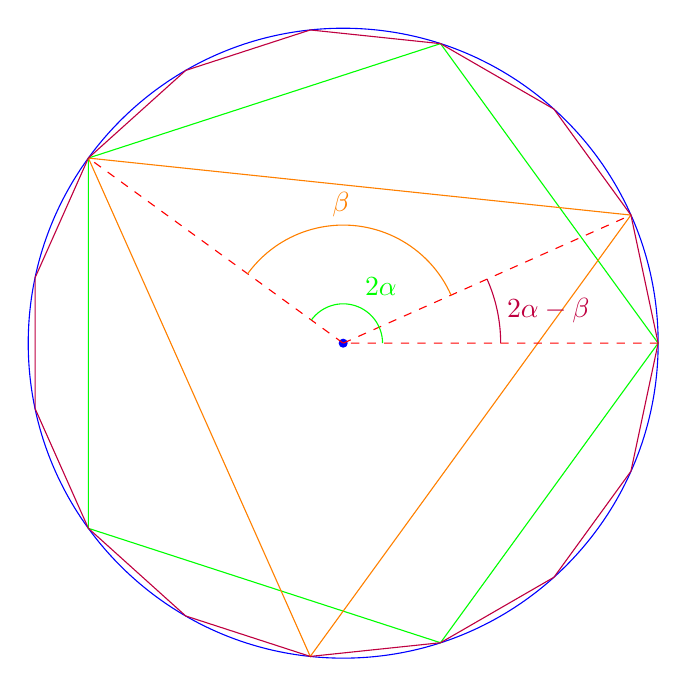
\begin{tikzpicture}
  \draw (0,0) circle(4)[color=blue];
  \draw[fill=black] (0,0) circle(.05)[color=blue];
  \draw[color=green]
  (4, 0) --
  (1.23606797749979,3.804226065180614) --
  (-3.236067977499789,2.351141009169893) --
  (-3.23606797749979,-2.351141009169892) --
  (1.23606797749979,-3.804226065180614) -- 
  (4,0);
  \draw[color=orange]
  (-3.236067977499789,2.351141009169893) -- (3.654181830570403,1.6269465723032)
  -- (-0.41811385307061,-3.978087581473093) --
  (-3.236067977499789,2.351141009169893);
  \draw[dashed,color=red]
  (4,0) -- (0,0) -- (-3.236067977499789,2.351141009169893);
  \draw[dashed,color=red]
  (0,0) -- (3.654181830570403,1.6269465723032);
  \draw[color=green] (.5,0) arc (0:72:.5) node[above right]{$2\alpha$} 
  arc (72:144:.5);
  \draw[color=orange] (1.370318186463901,0.6101049646137) arc (24:100:1.5)
  node[above right]{$\beta$} arc (100:144:1.5);

  \draw[color=purple] (2,0) arc (0:12:2)
  node[right]{$2\alpha-\beta$} arc (12:24:2);

  \draw[color=purple] (4,0) -- 
  (3.654181830570403,1.6269465723032)--
  (2.676522425435433,2.972579301909576) --
  (1.236067977499789,3.804226065180614) --
  (-0.41811385307061,3.978087581473093) --
  (-2.0,3.464101615137754) --
  (-3.236067977499789,2.351141009169893) --
  (-3.912590402935222,0.83164676327103) --
  (-3.912590402935222,-0.83164676327103) --
  (-3.236067977499789,-2.351141009169893) --
  (-2.0,-3.464101615137754) --
  (-0.41811385307061,-3.978087581473093) --
  (1.236067977499789,-3.804226065180614) --
  (2.676522425435433,-2.972579301909576) --
  (3.654181830570403,-1.6269465723032) --
  (4,0);
\end{tikzpicture}
\end{center}

En este ejercicio, hemos obtenido todos los $n$-gonos regulares que es
posible contruir con regla y compás, para $n \leq 16$. Gaus dio una construción
del heptadecágono regular ($n=17$ lados).

\subsection{Ejercicio 7 (Cuadriláteros)}

\begin{enumerate}
\item Un cuadrado de lado $a$ tiene perímetro $4a$ y área $a^2$. 
\item El perímetro del rombo es $4c$ y
  su areá es la mitad del rectángulo ázul, es decir $\frac{ab}{2}$.
\item La formula del perímetro es la misma que la del rectángylo: $2{(a+b)}$.
  Podemos cortar el triángulo rosa y mover esta parte para obtener un
  rectángulo de lados $a,h$ de misma área: $a \times h$.
\item El área del trapezoide es la mitad del paralelogramo:
  $\frac{{(a+b)} \times h}{2}$.
\end{enumerate}

\subsection{Ejercicio 8 (Triángulo)}

\begin{enumerate}
\item $a+b+c$
\item $3a$ (equilátero de lado $a$), $a+2b$ (isósceles de lado $a,b,b$)
  $a+b+\sqrt{a^2+b^2}$ (rectángulo de lados menores $a,b$),
  ${(2+\sqrt{2})}a$ (rectángulo isósceles de lados menor $a$).
\item Es la mitad del paralelogramo en la figura: $\frac{a \times h}{2}$.
\item Un triángulo rectángulo de lado menores $a,b$ (respectivamente
  rectángulo isósceles de lado menor $a$) es la mitad de un rectángulo de lado
  $a,b$ ((respectivamente de un cuadrado de lado $a$) y obtenemos
  $\frac{ab}{2}$ y $\frac{a^2}{2}$. En la formula general, $a$ es un lado menor
  y la altura $h$ el otro lado menor.

  Para un triángulo equilátero de lado $a$, el teorema de pitágoras da
  $h = \sqrt{a^2 - \left(\frac{a}{2}\right)^2} = \frac{\sqrt{3}}{2} a$ y
  entonces el área es $\frac{\sqrt{3}}{4} a^2$.
  
\end{enumerate}

\subsection{Ejercicio 9 (polígonos regulares, Arquímedes)}

\begin{enumerate}
\item Ver el Ejercicio 6:

\begin{center}
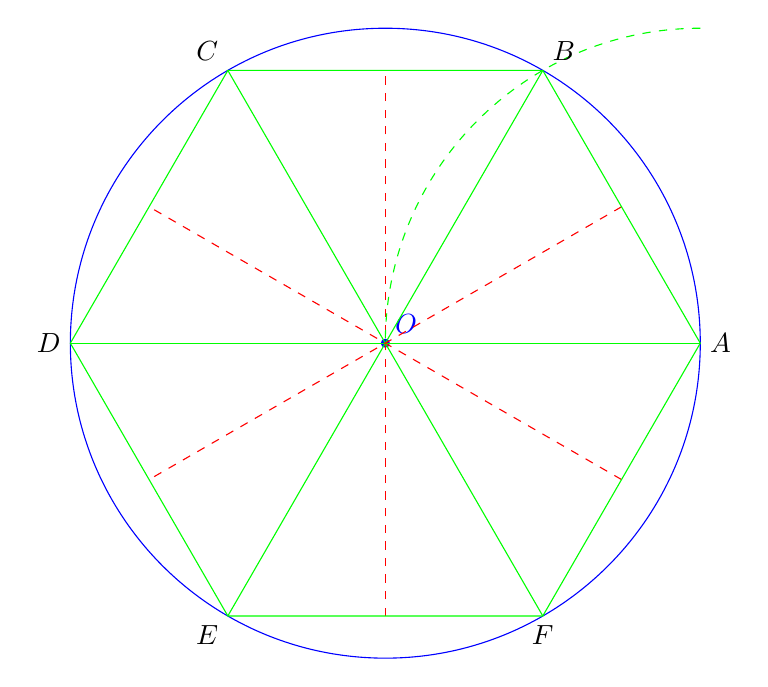
\begin{tikzpicture}
  \draw (0,0) circle(4)[color=blue];
  \draw[fill=black] (0,0) circle(.05)[color=blue] node[above right]{$O$};

  \draw (-4,0) -- (4,0)[color=green];
  \draw (0,-3.464101615137754) -- (0,3.464101615137754)[dashed,color=red];

  \begin{scope}[rotate around={60:(0,0)}]
  \draw (-4,0) -- (4,0)[color=green];
  \draw (0,-3.464101615137754) -- (0,3.464101615137754)[dashed,color=red];
  \end{scope}

  \begin{scope}[rotate around={120:(0,0)}]
  \draw (-4,0) -- (4,0)[color=green];
  \draw (0,-3.464101615137754) -- (0,3.464101615137754)[dashed,color=red];
  \end{scope}

  \draw (4,4) arc(90:180:4)[dashed,color=green];
  \draw (4,0) node[right]{$A$}
  -- (2,3.464101615137754)  node[above right]{$B$}
  -- (-2,3.464101615137754)  node[above left]{$C$}
  -- (-4,0)  node[left]{$D$}
  -- (-2,-3.464101615137754) node[below left]{$E$}
  -- (2,-3.464101615137754) node[below]{$F$}
  -- (4,0) [color=green];


\end{tikzpicture}
\end{center}


\item El hexágono tiene $6$ lados de longitud $R$ y entonces el
  périmetro es $6R$. Cómo en el ejercicio 8, 
  la longitud del apotema es $\frac{\sqrt{3}}{2} R$ y 
  la área es del hexágono
  es $6 \frac{\sqrt{3}}{4} R^2 = \frac{3 \sqrt{3}}{2} R^2$.
\item Eso es un hexágono de radio
  ${\frac{2}{\sqrt{3}} R}={\frac{2\sqrt{3}}{3} R}$ y entonces
  de périmetro $4 \sqrt{3} R$ y área $2 \sqrt{3} R^2$.
  Entonces $6R \leq P_C \leq 4 \sqrt{3} R$ y
  $\frac{3 \sqrt{3}}{2} R^2 \leq A_C \leq 2 \sqrt{3} R^2$.
\item $3 = \frac{6R}{2R} \leq \pi \leq \frac{4 \sqrt{3} R}{2R} = 2\sqrt{3} \approx 3.464101615137754$.
  Arquímedes utilizó $96$-gonos para obtener una mejor approximación
  $3.1408 \approx \frac{310}{71} \leq \pi \leq \frac{31}{7} \approx 3.1429$.
\item Si el polígono tiene $n$ lados de longitud $l$, su perímetro es $nl$.
  Su área se compone de $n$ tríangulos de lado $l$ y altura $h$ entonces
  es $n \frac{l \times h}{2} = \frac{nlh}{2}$.

\item El perímetro $nl$ se acerca de $P_C = 2 \pi R$, la altura $h$ se acerca
  de $R$. Entonces el área del polígono se acerca de
  $\frac{2 \pi R \times R}{2} = \pi R^2$. En efecto, podemos mostrar que
  el área de un círculo de radio $R$ es $A_C = \pi R^2$.
\end{enumerate}
